\section{Billedanalyse}

\begin{frame}
\frametitle{Billedanalyse}
\begin{itemize}
\item Kameraet kan give os et billede eller en videosekvens
\item Skal patienten selv tage billeder?
\item Ansigtsgenkendelse hjælper os til at tage et billede af brugeren uden vedkommende ved det

\end{itemize}
\end{frame}


\begin{frame}
\frametitle{Billedanalyse}
\begin{figure}
\centering
\begin{subfigure}[b]{0.45\textwidth}
	\centering

\includegraphics[width=\textwidth]{pupil-dilation}
\caption{Pupil reaktion.}
\end{subfigure}
~~~~
\begin{subfigure}[b]{0.45\textwidth}
	\centering
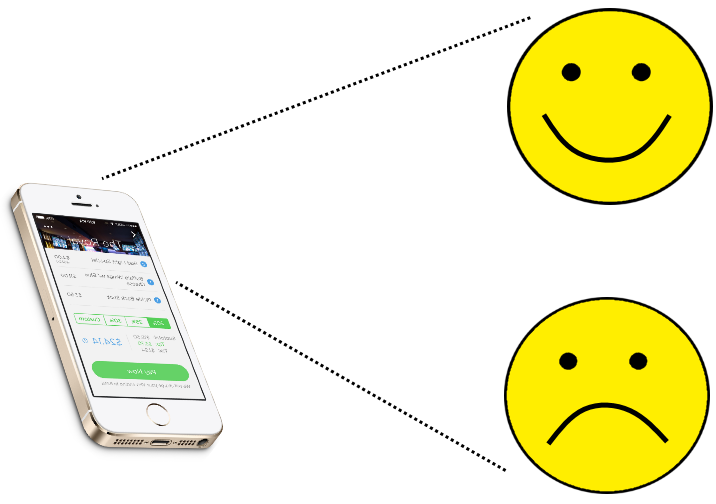
\includegraphics[width=\textwidth]{humoer}
\caption{Humør.}
\end{subfigure}
\caption{Idéer til brug af kameraet.}
\end{figure}

\end{frame}

\section{Accelerometer}
\begin{frame}
\frametitle{Accelerometer}
\end{frame}